\documentclass[conference]{IEEEtran}
\IEEEoverridecommandlockouts
% The preceding line is only needed to identify funding in the first footnote. If that is unneeded, please comment it out.
\usepackage{graphics} % for pdf, bitmapped graphics files
\usepackage{subfigure}
\usepackage{epsfig} % for postscript graphics files
\usepackage{mathptmx} % assumes new font selection scheme installed
\usepackage{times} % assumes new font selection scheme installed
\usepackage{amsmath} % assumes amsmath package installed
\usepackage{amssymb}  % assumes amsmath package installed
\usepackage{float}
\usepackage{multirow}
\usepackage{makecell}
\usepackage[section]{placeins}
\usepackage{comment}
%\floatBarrier
\usepackage{cite}
\usepackage{amsfonts}
\usepackage{algorithmic}
\usepackage{graphicx}
\usepackage{textcomp}
\usepackage{xcolor}
\def\BibTeX{{\rm B\kern-.05em{\sc i\kern-.025em b}\kern-.08em
    T\kern-.1667em\lower.7ex\hbox{E}\kern-.125emX}}
\begin{document}

\title{Reduction of Workflow Resource Consumption \\ Using a Density-based Clustering Model \\
%{\footnotesize \textsuperscript{*}Note: Sub-titles are not captured in Xplore and should not be used}
%\thanks{This work is funded by ???}
}

\author{
\IEEEauthorblockN{Qimin Zhang}
\IEEEauthorblockA{\textit{Key Laboratory of Space Utilization} \\
\textit{Chinese Academy of Sciences}\\
Beijing, China \\
zhangqimin16@csu.ac.cn}
\and
\IEEEauthorblockN{ Nathaniel Kremer-Herman}
\IEEEauthorblockA{\textit{Department of Computer Science and Engineering} \\
\textit{University of Notre Dame}\\
Notre Dame, US \\
nkremerh@nd.edu}
\and
\IEEEauthorblockN{Ben Tavor}
\IEEEauthorblockA{\textit{Department of Computer Science and Engineering} \\
\textit{University of Notre Dame}\\
Notre Dame, US \\
btovar@nd.edu}
\and
\IEEEauthorblockN{Douglas Thain}
\IEEEauthorblockA{\textit{Department of Computer Science and Engineering} \\
\textit{University of Notre Dame}\\
Notre Dame, US \\
dthain@nd.edu}

}

\maketitle

\begin{abstract}
Often times, a researcher running a parallel application will ask for orders of magnitude too few or too many resources to run their application. If the resource requisition is too small, the job may fail due to resource exhaustion; if it is too large, resources will be wasted though job may succeed. It would be ideal to achieve a near-optimal number of resources the application runs to ensure all jobs succeed and minimize resource waste. We present a strategy for solving the resource allocation problem: (1) resources consumed by each job are recorded by a resource monitor tool; (2) a density-based clustering model is proposed for discovering clusters in all jobs; (3) a maximal resource requisition is calculated as the ideal number of each cluster. We ran experiments with a synthetic workflow of homogeneous tasks as well as the bioinformatics tools Lifemapper, SHRIMP, BWA and BWA-GATK to capture the inherent nature of resource consumption of a parallel application, the clustering allowed by the model, and its usefulness in real applications.
\end{abstract}

\begin{IEEEkeywords}
density-based clustering, automatic resource allocation, resource consumption optimization.
\end{IEEEkeywords}

\section{Introduction}
High performance computing is an essential component of the scientific enterprise in fields as diverse as computer science, physics, biology, economics, and aerospace. Scientists use it to enable new discoveries, like discovering new galaxies in digital imagery, predicting the effect of new drugs using computational modeling, and many more. In high performance computing, researchers will often run a very large number of independent jobs across a large number of independent nodes (machines) [1].

In a parallel application, failed job caused by resource exhaustion will waste time and resources due to being returned and re-submitted. Thus, the user tend to submit jobs with a large resource requisition to ensure all jobs succeed[2]. However, one goal of high performance computing is to run a parallel application with maximal number of jobs completed over a long period of time and minimal resource consumption of jobs. Thus, researchers will often ask for how many resources (such as cores, memory, and disk) should be requested for each job.

In practice, a researcher running a parallel application will often have very little detailed information about per job. So it is generally difficult for users to do the resource allocations ideally when jobs consume various cores, disk, memory and other resources due to their functions and processing data. We call this the resource allocation problem: how should the user make resource allocation strategies without detailed information of per job so as to minimize the waste of their resource consumption?

Data mining-based algorithms are widely investigated in parallel applications to facilitate resource allocation and management. In [3], Menache et al. presented an online learning resource allocations to balance the computation cost and performance. It is based on the learning from the executing performance of prior job while collaborating history of spot prices and workload characteristics. In [4], Chen et al. presented a statistical model checker UPPAAL-SMC for optimizing and evaluating for cloud workflow resource allocation strategies. In [5], Xiong et al. proposed a cost-aware resource management system SmartLA using machine learning techniques for achieving the optimum profits. However, whether the prediction algorithm is nonlinear regression, statistical model or neutral network, the accuracy of the prediction model is not up to one hundred percent. Thus, at least a small number of jobs will fail due to the resource requisition is too small, which means their methods are generally not able to ensure all tasks succeed according to their resource allocation strategies.

Considering that sometimes users need to run the same workflow for multiple times or run a small application for testing before running the whole application we present a comprehensive solution to the resource allocation problem for minimizing the waste of resource consumption while running all jobs successfully. We extract features from data collected by a resource monitor tool, then we use a density-based clustering model for discovering clusters in a large number of jobs, calculating optimal resource requisition for each cluster to optimize resource management. Section 2 gives the background and an overview of our method. Section 3 formalizes our ideas, presenting the algorithm and structure of our density-based clustering model, and our parameters' value evaluation strategies. Section 4 evaluates our approach using resource consumption data collected from production workflows in domains of bioinformatics. We demonstrate that our resource allocation strategy leads to an overall decrease in resource consumption compared to fixed allocations under the richness of resource variations.

\section{Implementation}

\subsection{Background}

TWe use Makeflow [6] to test our approach, which is a workflow system designed to allow users to use workflows and make files. Makeflow interfaces with several different job processing systems for executing the jobs submitted to it. It can run jobs locally, or interface with Condor [7] or other systems. We run scientific workflows both locally and Condor to evaluate the behavior of our approach.

We assume a system composed of the following parts. The user provides a workflow description which indicates a set of jobs to be run, and the dependencies between them. A resource monitor tool [8] to monitor the computational resources of a process. It generates report files: a summary file with the maximum values of resource and time each job used, and monitors the maximum resources limit specified in the workflow file. If one of the resources goes over the limit, then the monitor terminates the task, including a report of the resource that was above the limit. Then the density-based clustering model do data clustering with all report files and the ideal resource allocation strategy is calculated, in terms of a quantity of cores, memory and disk. 

\subsection{Our approach}
The structure of our solution is shown in Fig. 1. When we run a parallel application, we use a resource monitor tool to observe, record, and enforce resource limits on jobs. These observations are used as data source for the next step.

A density-based clustering model is presented to do data clustering. We extract cores, disk, memory and wall-time data from report files as four-dimensional features of each job and specify weights for each dimension to represent the importance of each feature. Then we cluster data according to the density aggregation of each point (job). After clustering, we label each task with its specified cluster number and the maximum resources of each cluster is calculated in order to ensure no task would fail. In this way, we obtain the ideal number of cores, memory and disk of each cluster with their specified cluster label. 

We evaluate these techniques on a synthetic workflow of homogeneous tasks as well as the bioinformatiocs tools Lifemapper, SHRIMP, BWA and BWA-GATK. The experiments were designed to capture the inherent nature of resources consumption of a parallel application, the clustering allowed by the model, and its usefulness in real applications.

\begin{figure}[htbp]
\centering
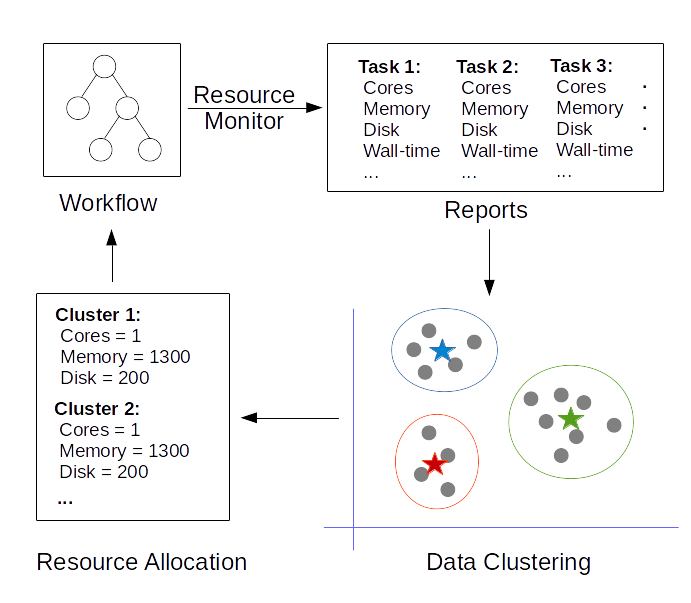
\includegraphics[width=3.2in]{./flow.png} 
\caption{System Components. The system consists of three main steps: (1) generate resource consumption reports, (2) data clustering with data collected by the resource monitor tool, (3) calculate ideal resource allocation strategy, then we re-run the workflow to measure the efficiency of our approach.}
\end{figure}

%%%%%%%%%%%%%%%%%%%%%%%%%%%%%%%%%%%%%%%%%%%%%%%%%%%%%%%%%%%%%%%%%%%%%%%%%%%%%%%%
\section{DENSITY-BASED CLUSTERING MODEL}
We present a density-based clustering model for discovering the inherent nature of jobs in parallel applications. In this section, we discuss the advantages of a density-based algorithm, model structure, crucial definitions, and strategy for selecting parameters in our clustering model.

\subsection{Clustering Algorithm}
The purpose we use clustering is to discover inherent clusters, or relationships within all tasks, and provide an ideal resource allocation strategy for users. However, usually, users do clustering with very few or no detailed information of each task. We assume that users are not always able to determine how many clusters should be in the parallel application. Moreover, the distribution of hundreds or thousands of jobs are not always able to have regular shapes like circles or squares. Actually, the distribution of all tasks in a parallel application often have various shape and size. Some classic clustering algorithms, for example, K-means [9] which clusters data by trying to separate samples in $n$ groups of equal variance, minimizing a criterion known as the inertia or within-cluster sum-of-squares, is limited by requiring the number of clusters to be specified in advance and its poor performance in unregulated shape. 

The density-based clustering algorithm [10] was selected in our strategy due to two main advantages: (1) clusters found by density can be any shape; (2) the number of clusters is not required to be specified primitively. The density-based clustering algorithm views clusters as areas of high density separated by areas of low density, so the shape of clusters depends on density differences between points, which means clusters are not required to be convex shaped that is required in K-means and other clustering algorithms. Also the number of clusters is determined by parameters in our algorithm, so the number of clusters is not required to be specified before clustering.

\subsection{Feature Extraction} 
We consider the clustering results related to a job in four stages:(1) how many cores the job used, (2) how much memory the job used, (3) how much disk the job used, and (4) how much wall-time the job used. Cores, memory and disk are three main parameters for resource allocations, so they are selected as parts of features. Wall-time is also selected as a feature for measuring the job size or function type.

The resource monitor provides summary files about computational resources of per task, so all these summary files are used to be data source of our clustering model. In our method, we extract features from reports, in terms of the quantity of cores, memory, disk and wall-time consumed by each task.

\subsection{Model Parameters}
Cores, memory, disk and wall-time are extracted as features of each single task, and we set weights to these four features. Then we provide a clustering model based on density for discovering clusters in large spatial databases. The central component is the concept of core samples, which are samples that are in areas of high density. A cluster is therefore a set of core samples, each close to each other (measured by some distance measure) and a set of non-core samples that are close to a core sample (but are not themselves core samples).

The following are several crucial definitions in the density-based clustering model:

\begin{itemize}

\item \textbf{\emph{distance}}. The definition of distance in our method is weighted-Minkowski. The distance $D(X,Y)$ between two points $X=(x_1, x_2, x_3, x_4)$ and $Y=(y_1, y_2, y_3, y_4)$ is defined as:
$$
D(X,Y)=({\sum_{i=1}^{4}w\times{\left|{x_i-y_i} \right|^p}})^{(1/p)} \eqno{(1)}
$$
$w$ represents the weights, we use the familiar Euclidean distance ($p$ = 2), and the distance $D(X,Y)$ also represents inherent relationship or similarity between two points.
\item \textbf{\emph{weights}}. Weights represent the importance of features(or axes). In our method, memory was considered to be the most representative and important feature of task attributes, so memory was given the largest weight. Weights of cores, memory, disk and wall-time were set to be 0.1, 0.7, 0.1, 0.1 respectively.
\item \textbf{\emph{eps}}. The maximum distance between two samples for them to be considered as in the same cluster(or neighborhood). If the \emph{eps} is too small, we will get too many clusters; on the other hand, if the \emph{eps} is too large, we will get too few clusters due to points would be considered in the same cluster when their distance is smaller than \emph{eps}. The value of \emph{eps} should be modified in different applications to achieve better performance.
\item \textbf{\emph{minimal samples}}. The minimal number of sample in a cluster. If \emph{minimal samples} was set to be more than 1, which means each cluster has two points at least, the point isolated with any other points would be seen as noise. To be noted, each job should have its cluster label to calculate its ideal resource requisition. Thus, \emph{minimal samples} is set to be 1 in our method.

\end{itemize}

After data clustering, we are able to obtain several clusters, label all points(tasks) with cluster numbers and calculate the maximum resources (cores, memory, disk) of each cluster. As show in Fig. 2, we provide the clustering result of BWA-GATK-workflow [11] as an example. This workflow is an bioinformatics example of using Makeflow to parallelize the Burroughs-Wheeler Alignment and Genome Analysis Toolkit (BWA-GATK) tool.

\begin{figure}[htbp]
  \centering 
  \subfigure[Before Clustering]{ 
    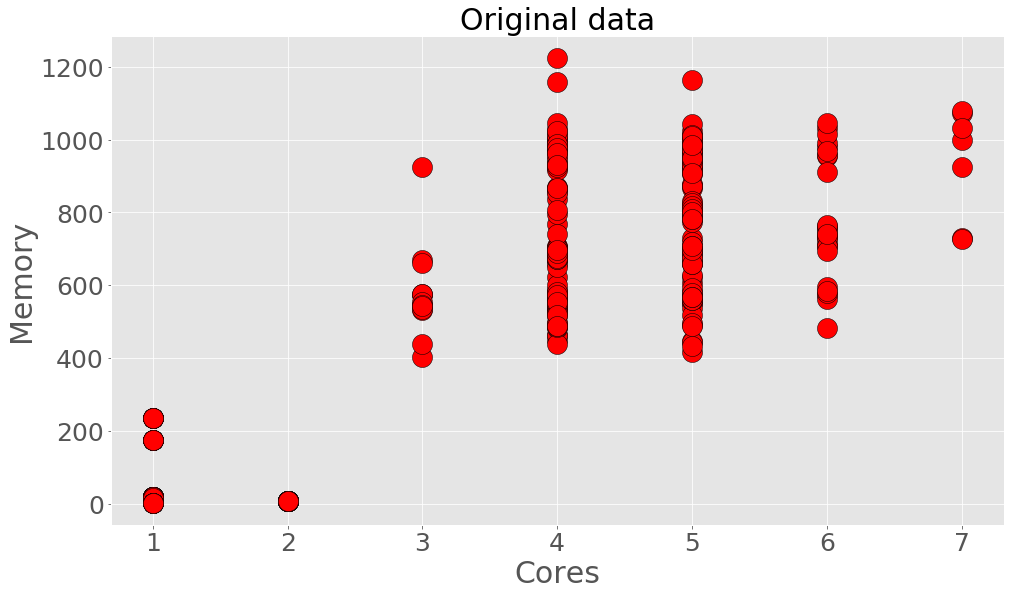
\includegraphics[width=3.2in]{./bwa-gatk-original.png} 
  } 
  \subfigure[After Clustering]{ 
    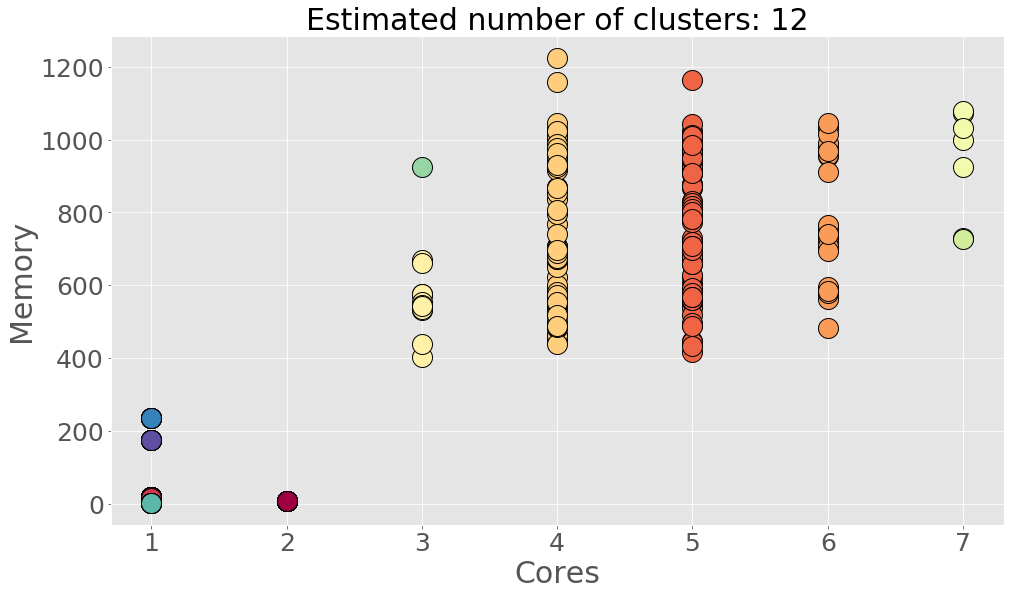
\includegraphics[width=3.2in]{./bwa-gatk.png} 
  } 
  \caption{Clustering result of BWA-GATK. The density-based clustering model used in our method is four dimensional, in terms of weighted cores, memory, disk and wall-time. Four dimensional distribution is hard to express in a figure. So we present the clustering result in two dimension: cores, and memory.} 
\end{figure}

Every point represents a task, and in Fig. 2 (b) different colors represent different clusters. So as shown in Fig. 2, all tasks have their own cluster labels, which means they have a specified number of resources according to their labels. In each cluster, the maximal resources consumed by tasks, in terms the quantity of cores, memory, and disk, are selected to be the ideal value of resources limitation. Then we are able to do an optimal resource allocations of all jobs in the parallel application.

\subsection{Parameters Selection Strategy}
We have discussed the algorithm and structure of the density-based clustering model, also the value of \emph{weights}, \emph{minimal samples}, and \emph{distance} have been discussed above, however, the value of \emph{eps} is required to be modified in individual application in order to performance better.

How to select the value of parameters in clustering model and how to evaluate the performance of clustering model with different value? We present two ways to evaluate the result of clustering: (1) compare with workflow structure, the higher the similarity is, the better we think of the performance, (2) use Calinski-Harabaz index [12], the higher the score is, the better we think of the performance.

\subsubsection{Compare with Workflow Structure}
Comparing the command line with the clustering result is a relatively simple method and this method is suitable for workflow with simple structure, such as SHRIMP-workflow [13]. In this method, the structure of workflow or the command line is used to be the ground truth of clustering results. If the clustering result is similar with the workflow structure, we think the clustering model have a good performance. So when the value of \emph{eps} make the clusters match best with the workflow structure, this value will be selected as the optimal one. As shown in Fig. 3, we use SHRIMP-workflow as an example, and present a best match between clustering result and the visualization of workflow structure. We present the figure in two axes, memory and disk, due to the value of cores consumption of all tasks in this workflow are 1. 

\begin{figure}[htbp]
  \centering 
  \subfigure[Clustering Result]{ 
    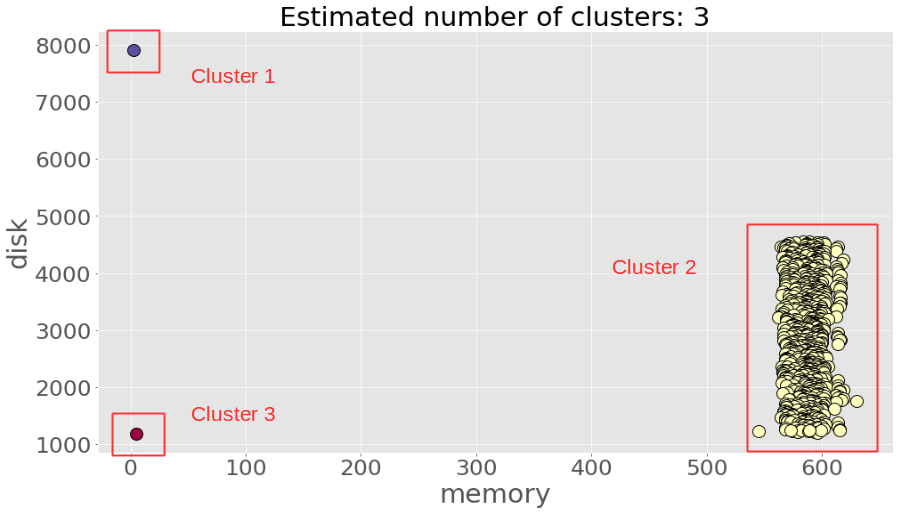
\includegraphics[width=3.2in]{./shrimpcluanno.png} 
  } 
  \subfigure[Workflow Structure]{ 
    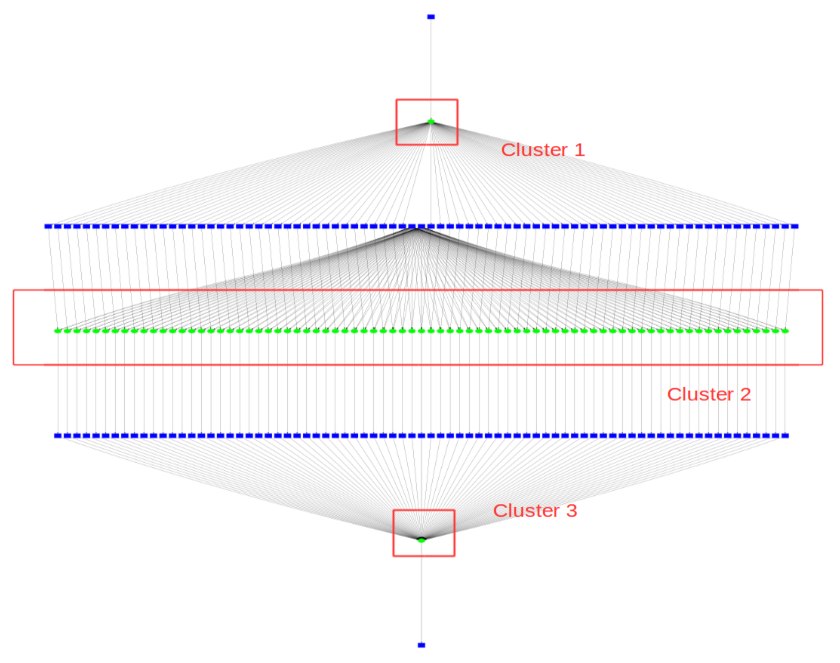
\includegraphics[width=3.2in]{./shrimpwork.png} 
  } 
  \caption{Match Performance for SHRIMP-workflow. SHRIMP-workflow is a bioinformatics workflow and the workflow structure graph shown clearly to show the general structure. The corresponding cluster labels: cluster 1, cluster 2, cluster 3, show the high matching performance of our clustering model and the real structure. } 
\end{figure}

As shown in Fig. 3, this workflow has three layers, and the clustering model also found three clusters. Meanwhile, corresponding clusters between Fig. 2(a) and (b) includes same tasks. So we think the clusters obtained by clustering model match perfectly with the workflow structure, and the value of \emph{eps} in this model is the optimal number.

\subsubsection{Index evaluation}
When the workflow structure is too complex or users do not have detailed information about commands, the Calinski Harabaz index can be used to evaluate the model, where a higher Calinski Harabaz score relates to a model with better defined clusters. The definition of C-H score is: for $k$ clusters, the C-H score $s$ is given as the ratio of the between-clusters dispersion mean and the within-cluster dispersion:
$$
s(k)=\frac{Tr(B_k)}{Tr(W_k)}\times\frac{N-k}{k-1}\eqno{(2)}
$$
where ${Tr(A}$ represents the matrix trace of matrix $A$, $B_K$ is the between group dispersion matrix to measure the dispersion degree between different clusters, and $W_K$ is the within-cluster dispersion matrix to measure the similarity of points within the same cluster, and they are defined by:
$$
W_K=\sum_{q=1}^{k}\sum_{x\in{C_q}}(x-c_q)(x-c_q)^T\eqno{(3)}
$$
$$
B_K=\sum_{q}n_q(c_q-c)(c_q-c)^T\eqno{(4)}
$$
with $N$ be the number of points in our data, $C_q$ be the set of points in cluster $q$, $c_q$ be the center of cluster $q$, $c$ be the center of $E$, $n_q$ be the number of points in cluster $q$.

As shown in Fig. 4, \textbf{BWA-GATK-workflow} has a relatively complex structure with many layers, which means it is unrealistic for users compare the clustering result with workflow structure. Thus, we use C-H score to select an ideal value of \emph{eps}. In this method, we think the value provides the highest C-H score is the optimal number. Use \textbf{BWA-GATK-workflow} as an example, we present the relationship between different value of \emph{eps} and its C-H score.

\begin{figure}[htbp]
\centering
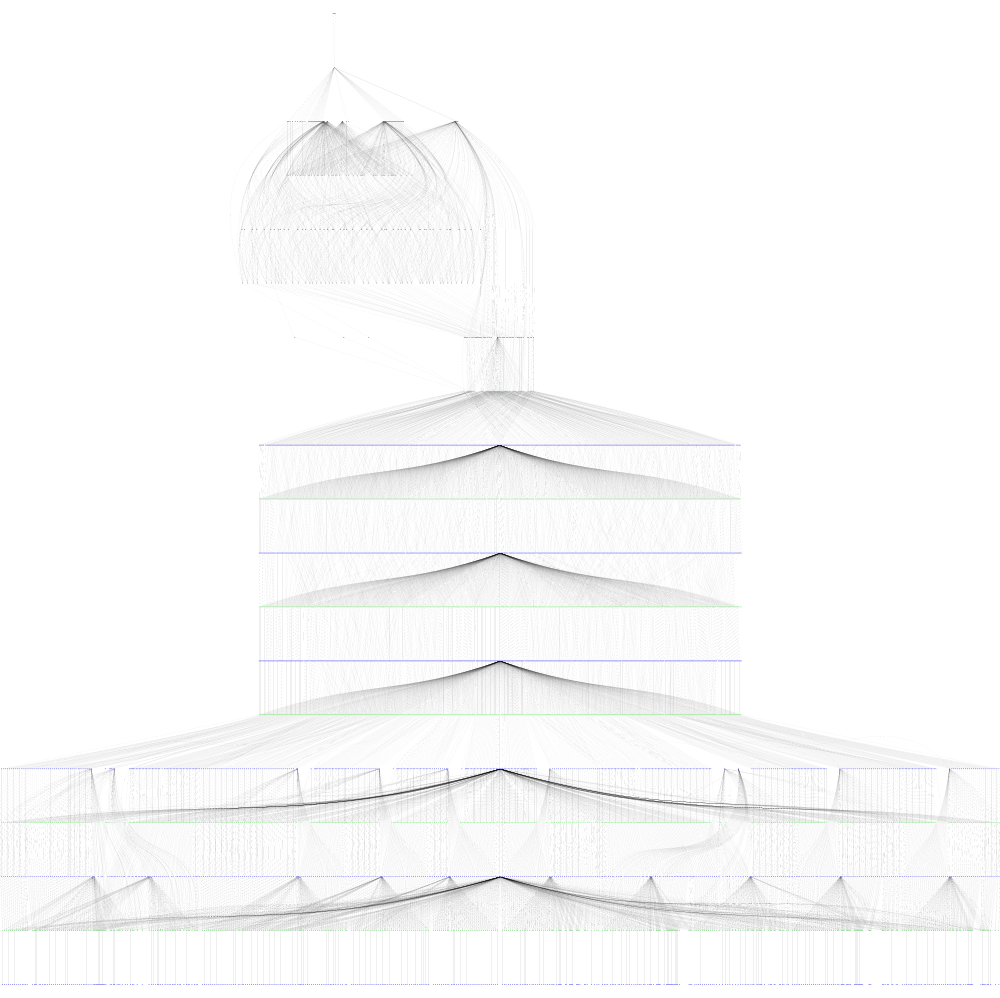
\includegraphics[width=3in]{./bwa-gatkworkflow.png} 
\caption{Structure of BWA-GATK-workflow. BWA-GATK-workflow is a bioinformatics workflow that performs genotyping of sequences related to the oak tree.}
\end{figure}

As shown in Fig. 5, C-H score fluctuate with different value of \emph{eps}. When the \emph{eps} is changed from 60 to 220, the C-H score first increases and then decreases, and the highest score is 1180, when \emph{eps} is 160. So in this workflow, we select 160 as the optimal value of \emph{eps}. When \emph{eps} is selected, the number of clusters $k$ will be determined in the clustering model. In this workflow, the number of clusters in is twelve, and the clustering result is shown in Fig. 2.

In BWA-GATK workflow, we use C-H score to find the optimal parameter value for the clustering model. However, it should be noted that the optimal value we find is a local optimal number rather than a global optimal number due to it is highly impossible for users to text all values from zero to infinity. Thus, we give a relatively sufficient number of values for parameters, and then we use C-H index for finding the optimal one.

\begin{figure}[htbp]
\centering
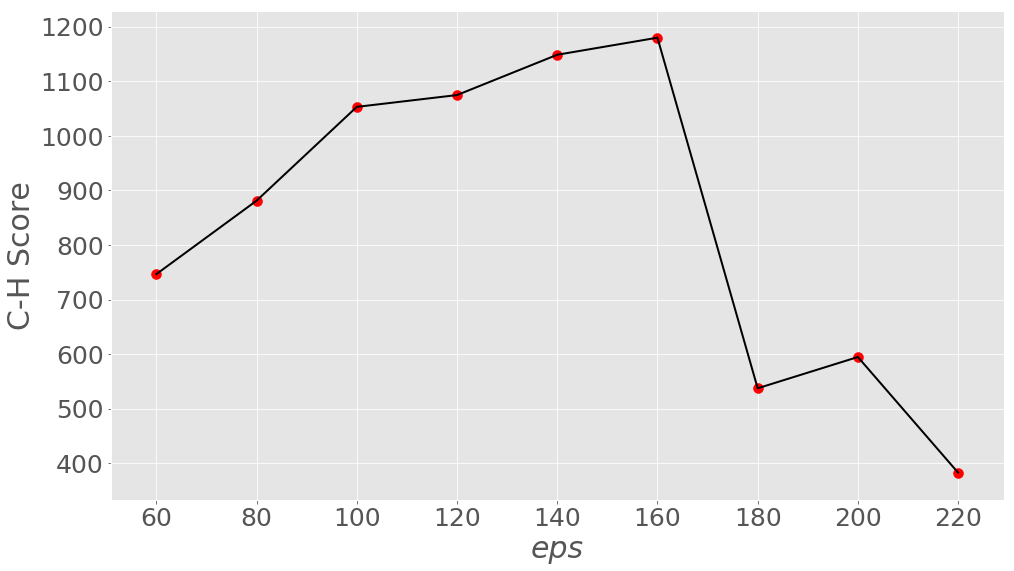
\includegraphics[width=3.2in]{./epsandscore.png} 
\caption{\emph{eps} and C-H Score. We measure the C-H score of various \emph{eps} from 60 to 220 with each 20 intervals. Each red scatter point has its related C-H score.}
\end{figure}


%%%%%%%%%%%%%%%%%%%%%%%%%%%%%%%%%%%%%%%%%%%%%%%%%%%%%%%%%%%%%%%%%%%%%%%%%%%%%%%%
\section{EVALUATION}
To evaluate our method, we apply it to data collected from production workflows runs on local machine and Condor batch system. For each job in a workflow, we use resource monitor tool to produce a summary file about how many resources consumed by each job. Using this data, we use density-based clustering model for labeling each task with its cluster number, calculating the maximal resources consumed by tasks in each cluster. Thus, we obtain an ideal resource allocation strategy. Then we re-run the workflow with new resource allocation strategy, and capture the cores, memory, disk, and wall-time consumed by each job. Finally, we compare two resource consumption reports described above and analyze cores saving, memory saving, disk saving and time saving of each workflow.

We evaluate these results on four different applications:

\textbf{Lifemapper-workflow} [14]consists of three steps: pre-processing, maxent, and projection. This workflow produce the most interesting results due to the real data it used, which leads to the various resource consumption reports when we run the same Lifemapper- workflow for multiple times. Thus, we run it for three times, and use all reports captured in these three times to get a more adaptive resource allocation strategy.

\textbf{SHRIMP-makeflow} consists of 763 jobs, divided in three steps: split, analysis, and join. The structure of this workflow is relatively simple, which has discribed in Section 3.4.

\textbf{BWA-makeflow} [15] is a bioinformatics workflow build on the Burrows Wheeler Alignment(BWA) tool, and it consists of 102 jobs, divided three steps: split, analysis, and join. Thus, the structure of this workflow is relatively simple, we analyze this workflow and do clustering in the same way as SHRIMP-workflow described in Section 3.4.

\textbf{BWA-GATK-makeflow} is a bioinformatics workflow that parallelize the Burroughs-Wheeler Alignment and Genome Analysis Toolkit (BWA-GATK) tool. The structure of this workflow is the most complex one in these five workflows.


\subsection{Improvement Index}
We analyze the reduction of resource consumption in four stages: time saving, cores saving, memory saving and disk saving, their definitions are described in the following:

\begin{itemize}
\item \textbf{\emph{time saving}} represents the decrease of running time.  $t$ is the number of cores consumed for running the workflow, then cores saving $t_s$ is define as::
$$
t_s=(t_b-t_a)/t_b\times100\%\eqno{(5)}
$$
$t_b$ is time consumed before clustering, $t_a$ is time consumed after clustering.

\item \textbf{\emph{cores saving}} represents the decrease of cores consumption. $c$ is the number of cores consumed for running the workflow, then cores saving $c_s$ is define as:
$$
c_s=(c_b-c_a)/c_b\times100\%\eqno{(6)}
$$
$c_b$ is the number of cores consumed before clustering, $c_a$ is the number of cores consumed after clustering.

\begin{figure*}
\centering
\begin{tabular}{r|cccc|cccc}
\hline
\multirow{3}{*}{Lifemapper} & \multirow{3}{*}{Job} & \multicolumn{3}{c|}{Resource Allocations} & \multicolumn{4}{c}{Resource Consumption}\\
& & cores & memory(GB) & disk(GB) & time(s) & cores & memory(GB.min) & disk(GB.min) \\ 
\hline
First run & 153 & 8 & 8000 & 50000 & 1394 & 1224 & 539 & 3370 \\
Second run & 153 & 4 & 8000 & 50000 & 542 & 612 & 406 & 2540 \\
Third run & 153 & 2 & 8000 & 50000 & 246 & 306 & 293 & 1833 \\
\hline
\multirow{6}{*}{After clustering} & \multirow{6}{*}{153} & \multicolumn{3}{c|}{cluster 1: Preprocessing} & \multirow{6}{*}{212} & \multirow{6}{*}{255} & \multirow{6}{*}{149} & \multirow{6}{*}{112}\\
&& 1 & 100 & 3000\\
&& \multicolumn{3}{c|}{cluster 2: Maxent}\\
&& 2 & 5000 & 3000\\
&& \multicolumn{3}{c|}{cluster 3: Projection}\\
&& 2 & 1500 & 3000\\
\hline
\end{tabular}
\caption{Resource consumption for Lifemapper-workflow}
\end{figure*}

\begin{figure}[t]
  \centering 
  \subfigure[Workflow Structure]{ 
    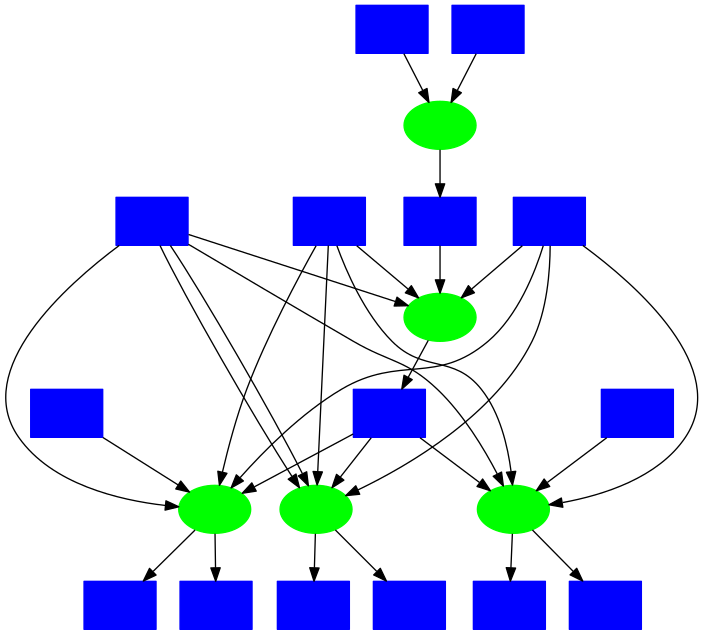
\includegraphics[width=2.6in]{./lifemapper.png} 
  } 
  \subfigure[Clustering Result]{ 
    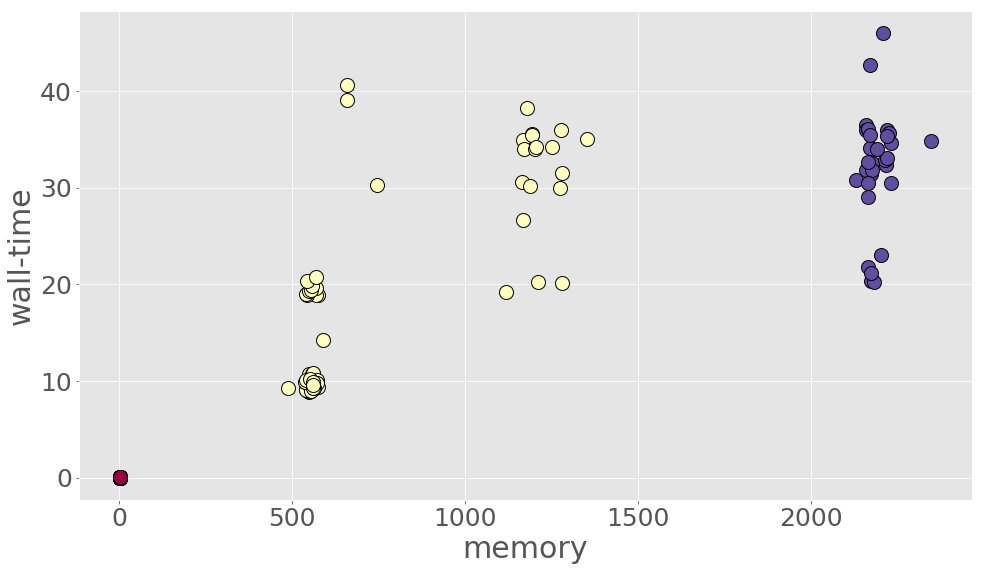
\includegraphics[width=3.2in]{./Lifemapper.png} 
  } 
  \caption{Clustering result for Lifemapper. We use four features to cluster data. Considering four dimensional distribution is hard to express in a graph, we present the clustering result in two dimension: memory and wall-time.}
\end{figure}

\begin{figure}[htbp]
\centering
\begin{tabular}{r|cccc}
\hline
\multirow{2}{*}{Lifemapper} & \multicolumn{4}{c}{Resource Saving}\\
& time & cores & memory & disk\\
\hline
$1^{st}$ run &  84.79$\%$ & 79.17$\%$ & 72.36$\%$ & 96.68$\%$\\
$2^{nd}$ run &  60.89$\%$ & 58.33$\%$ & 63.30$\%$ & 95.59$\%$\\
$3^{rd}$ run &  13.82$\%$ & 16.67$\%$ & 49.15$\%$ & 93.89$\%$\\
\hline
\end{tabular}
\caption{Resource saving for Lifemapper-workflow.}
\end{figure}


\item \textbf{\emph{memory saving}} represents the decrease of memory consumption. $m$ is the number memory(GB.min) consumed for running the workflow, we find the $m$ to be:
$$
m=\sum_{i=1,2,3...} t_i\times m_i
$$
$i$ is the number of task, so the memory saving $m_s$ is define as:
$$
m_s=(m_a-m_b)/c_1\times100\%\eqno{(7)}
$$
$m_a$ is memory consumed before clustering, $m_b$ is memory consumed after clustering.

\item \textbf{\emph{disk saving}} represents the decrease of disk consumption. $d$ is the number disk(GB.min) consumed for running the workflow, we find the $s$ to be:
$$
d=\sum_{i=1,2,3...} t_i\times m_i
$$
$i$ is the number of task, so the disk saving $m_s$ is defined as:
$$
d_s=(d_a-d_b)/c_1\times100\%\eqno{(8)}
$$
$d_a$ is disk consumed before clustering, $d_b$ is disk consumed after clustering.
\end{itemize}

\subsection{Offline Analysis}
We applied the density-based clustering model to all four workflows and compare the resource consumptions before clustering and after clustering. The results are used to demonstrate the efficiency improvements with our method. We show the results in Fig.s 6, 7, 8 for Lifemapper-workflow, and show the results in Fig.9, 10, 11 for BWA-workflow, SHRIMP-workflow, and GWA-GATK-workflow, respectively.

Lifemapper-workflow provides an interesting result. If users run the same workflow for multiple times, they may get different output due to the special real data this workflow used. As shown in Fig. 6, it consists of three steps, and each step contains 51 jobs. We run this workflow for three times, and we find that tasks in the second step Maxent consume various resources between each time. For example, the task No.68 consumes 2166 GB memory in the first run, but it consumes 1357 GB memory in the second run. Thus we use reports from all three times and use the maximal reports of each task, and then we do the clustering for finding ideal clusters. We use the strategy described in Section 3.4.1 to find the ideal parameters' value and the clustering result is shown in Fig. 7.

%%%%%%%%%%%%%%%%%%%%%%%%%%%%%%%%%%%%%%%%%%%%%%%%%%%%%%%%%%%%%%%%%%%%%%%%%%%%%%%% workflow %%%%%%%%%%%%%%%%%
\begin{figure*}[t]
  \centering 
  \subfigure[SHRIMP-workflow]{ 
    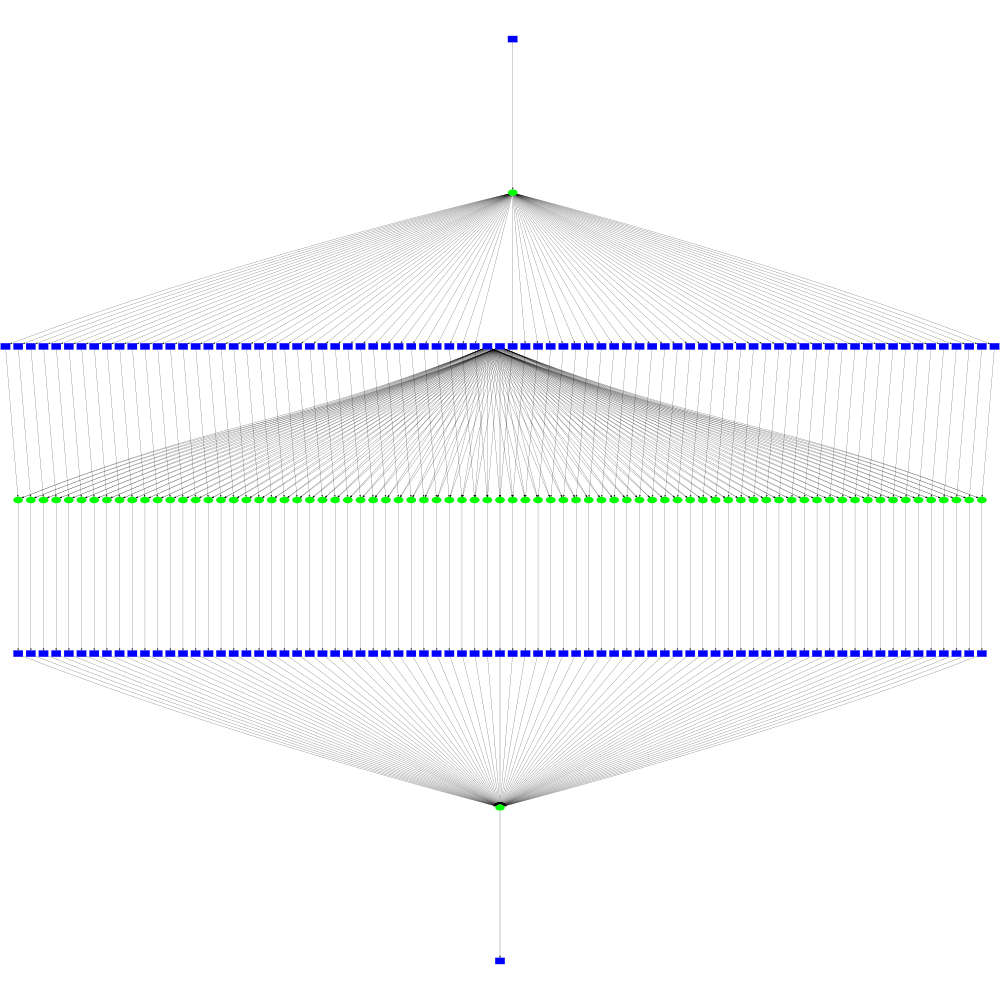
\includegraphics[width=2.2in]{./shrimp-workflow.png} 
  } 
  \subfigure[BWA-workflow]{ 
    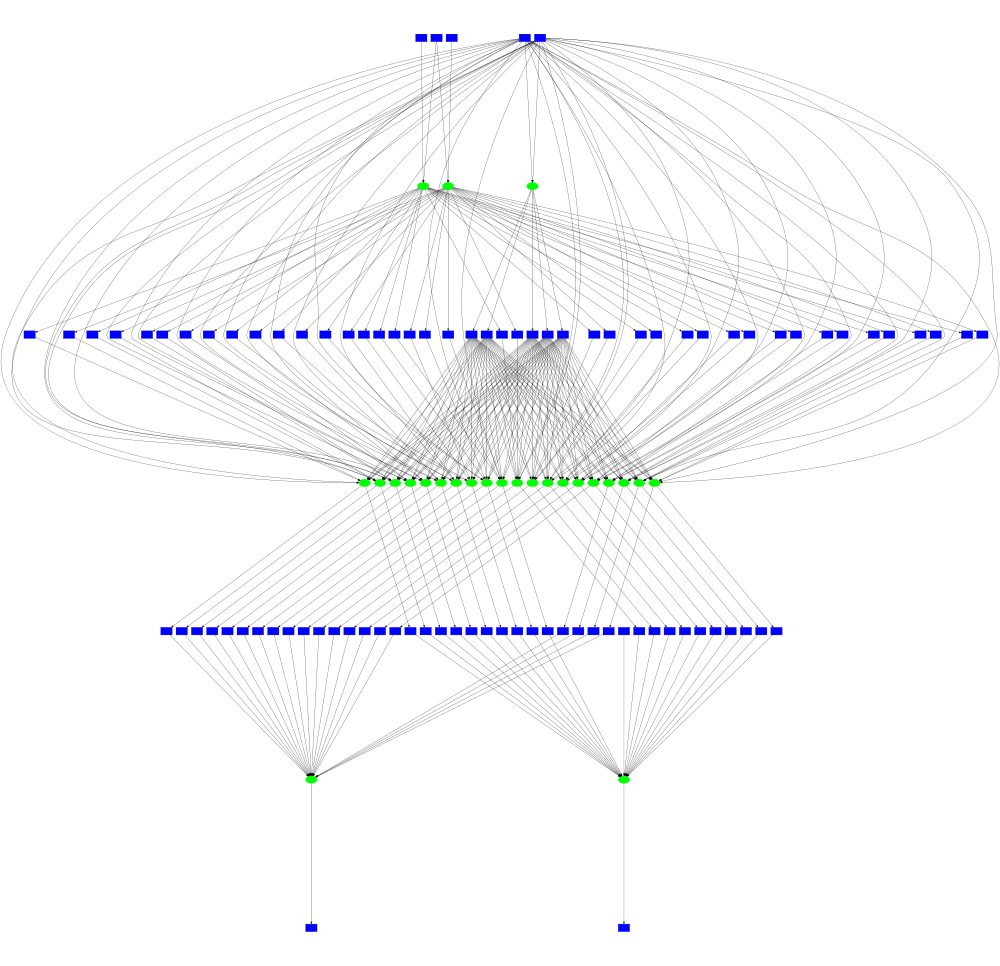
\includegraphics[width=2.2in]{./bwa-workflow.png} 
  } 
    \subfigure[BWA-GATK-workflow]{ 
    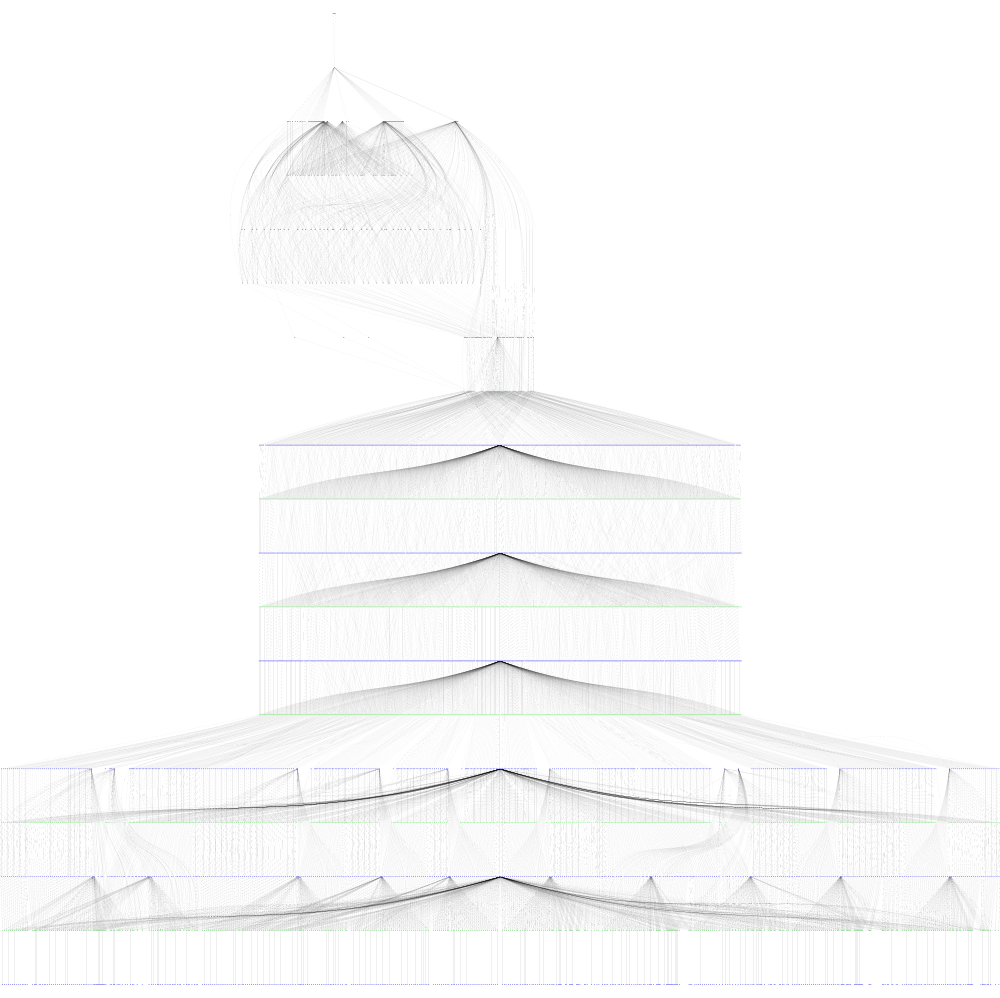
\includegraphics[width=2.2in]{./bwa-gatkworkflow.png} 
  } 
  \caption{Visilization for scitific workflows} 
\end{figure*}
%%%%%%%%%%%%%%%%%%%%%%%%%%%%%%%%%%%%%%%%%%%%%%%%%%%%%%%%%%%%%%%%%%%%%%%%%%%%%%%% clustring %%%%%%%%%%%%%%%%%
\begin{figure*}[t]
  \centering 
  \subfigure[SHRIMP-workflow]{ 
    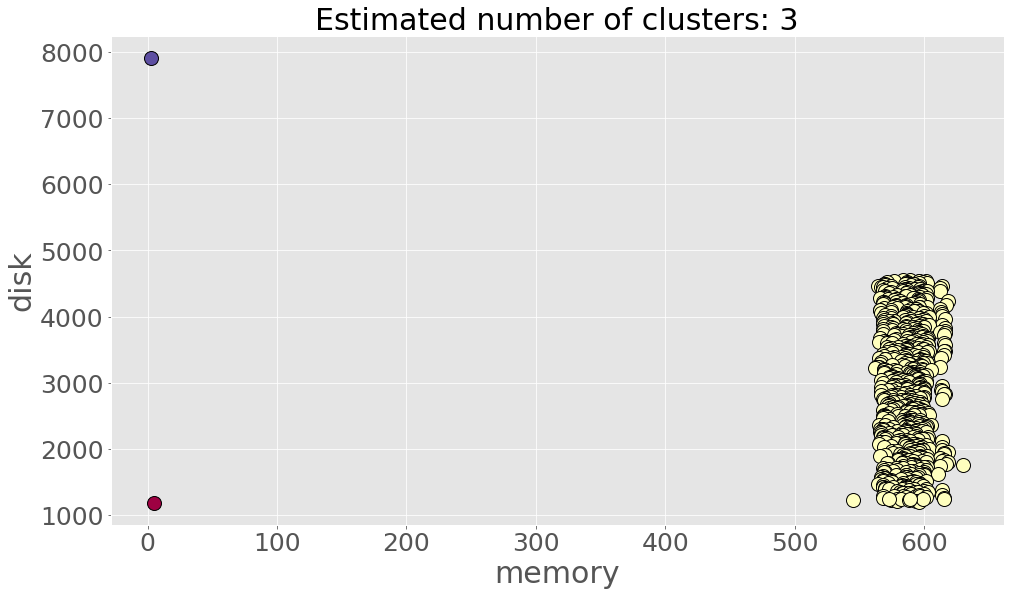
\includegraphics[width=2.2in]{./shrimp-clustering.png} 
  } 
  \subfigure[BWA-workflow]{ 
    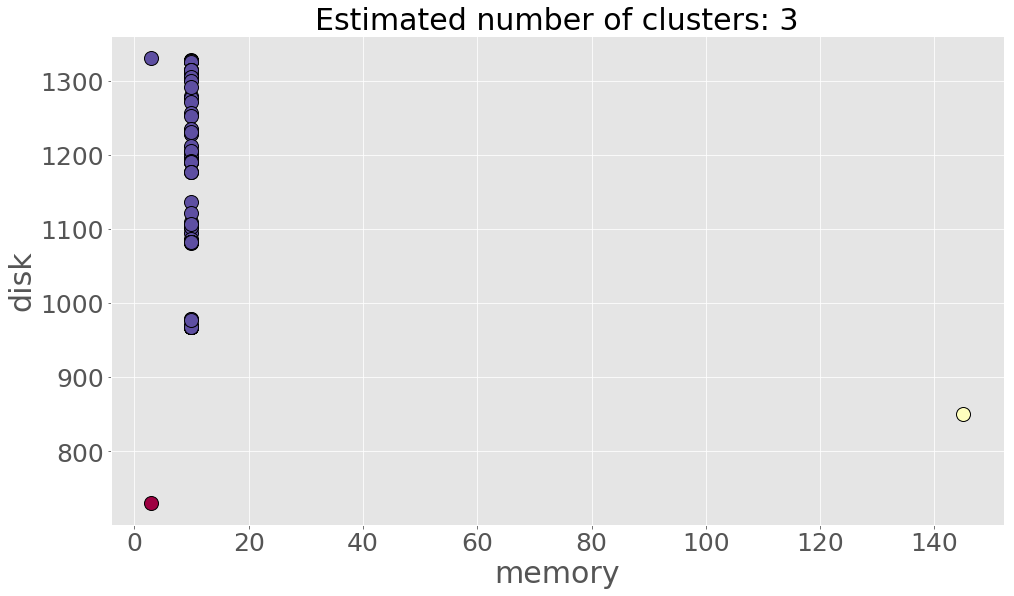
\includegraphics[width=2.2in]{./bwa-clustering.png} 
  } 
    \subfigure[BWA-GATK-workflow]{ 
    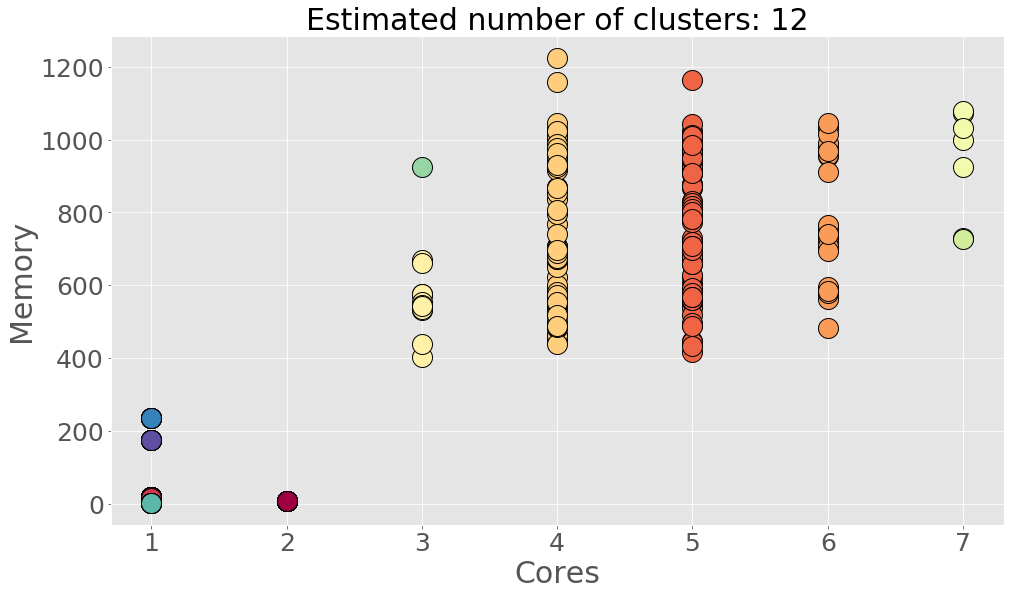
\includegraphics[width=2.2in]{./bwa-gatk.png} 
  } 
  \caption{Clustering results for scitific workflows. We use four features to cluster data in SHRIMP, BWA, BWA-GATK workflows. To show the clustering results clearly, we present the clustering results in two dimension: memory, and disk. Comparing corresponding workflows in Fig. 9 and Fig. 10, we are able to visualize the relation of real workflow structure and clustering result.} 
\end{figure*}
%%%%%%%%%%%%%%%%%%%%%%%%%%%%%%%%%%%%%%%%%%%%%%%%%%%%%%%%%%%%%%%%%%%%%%%%%%%%%%%% table %%%%%%%%%%%%%%%%%
\begin{figure*}[t]
  \centering 
\begin{tabular}{r|ccccccccc}
\hline
\multirow{2}{*}{workflow} & \multirow{2}{*}{category} & \multirow{2}{*}{job} & \multicolumn{4}{c}{resource allocations} & \multicolumn{3}{c}{resource consumption}\\
&&& cluster & cores & memory & disk & cores & memory & disk\\ 
&&&&& (GB) & (GB) & & (GB.min) & (GB.min)\\
\hline
\multirow{4}{*}{SHRIMP} & w/o clustering & 763 & 1 & 2 & 8000 & 50000 & 1526 & 18703 & 116892\\
& \multirow{3}{*}{with clustering} & \multirow{3}{*}{763} & 1 & 1 & 100 & 1300 & \multirow{3}{*}{763} & \multirow{3}{*}{1845} & \multirow{3}{*}{9238}\\
&&& 2 & 1 & 1000 & 5000\\
&&& 3 & 1 & 100 & 10000\\
\hline
\multirow{4}{*}{BWA} & w/o clustering & 102 & 1 & 2 & 2048 & 2048 & 204 & 8.78 & 8.78\\
& \multirow{3}{*}{with clustering} & \multirow{3}{*}{102} & 1 & 1 & 10 & 800 & \multirow{3}{*}{102} & \multirow{3}{*}{0.40} & \multirow{3}{*}{4.23}\\
&&& 2 & 1 & 200 & 1000\\
&&& 3 & 1 & 10 & 1400\\
\hline
\multirow{13}{*}{BWA-GATK} & w/o clustering & 530 & 1 & 8 & 8000 & 10000 & 4240 & 4287 & 5359\\
& \multirow{12}{*}{with clustering} & \multirow{12}{*}{530} & 1 & 2 & 100 & 300 & \multirow{12}{*}{1734} & \multirow{12}{*}{215} & \multirow{12}{*}{278}\\
&&& 2 & 1 & 100 & 300\\
&&& 3 & 5 & 1500 & 100\\
&&& 4 & 6 & 1500 & 100\\
&&& 5 & 4 & 1500 & 100\\
&&& 6 & 3 & 1000 & 100\\
&&& 7 & 7 & 1500 & 100\\
&&& 8 & 7 & 1000 & 100\\
&&& 9 & 3 & 1200 & 100\\
&&& 10 & 1 & 100 & 3500\\
&&& 11 & 1 & 500 & 3500\\
&&& 12 & 1 & 300 & 2000\\
\hline
\end{tabular} 
\caption{Clustering results for scitific workflows}
\end{figure*}

\begin{figure}[h]
  \centering 
\begin{tabular}{rccc}
\hline
\multirow{2}{*}{workflow} & \multicolumn{3}{c}{resource saving}\\
& cores & memory & disk\\
\hline
SHRIMP & 50.00$\%$ & 90.14$\%$ & 92.10$\%$\\
BWA & 50.00$\%$ & 95.44$\%$ & 51.82$\%$\\
BWA-GATK & 59.10$\%$ & 94.98$\%$ & 94.81$\%$\\
\hline
\end{tabular} 
\caption{Clustering results for scitific workflows}
\end{figure}

As shown in Fig. 7, we obtain three clusters and each cluster contains the same task with their corresponding steps. So we use this clustering model and calculate the max number of resources of each cluster in order to gain the ideal resource allocations. In practical application, we add a little more to the number we get to make sure all task succeed. Then we re-run the lifemapper-workflow and the results of resource saving are shown in Fig. 8. We run Lifemapper locally, so time saving is the reduction of running time for the whole workflow.

We can note that the time saving corresponds closely to the cores saving. The reason is that task would not run faster with more cores, but too many cores requisition will increase the waiting time of the following tasks. So when we use new resource allocations, in which we set cores requisition to 1 rather than 2, we decrease the waiting time for tasks. Thus, the time saving and cores saving is similar and all range from about 80$\%$ to about 15$\%$. The results also show obvious memory saving and disk saving, the least memory saving is 49.15$\%$ and the least disk saving 93.89$\%$. We observe a very noticeable resource saving with our method.

%%%%%%%%%%%%%%%%%%%%%%%%%%%%%%%%%%%%%%%%%%%%%%%%%%%%%%%%%%%%%%%%%%%%%%%%%%%%%%%% Shrimp %%%%%%%%%%%%%%%%%
We also applied our method to SHRIMP-workflow, BWA-workflow, and BWA-GATK-workflow. we show the visilazation of their structure, the clustering results, and the resource saving results in Fig. 9, 10, 11, respectively. In all these four workflow experiments, we compara the resource consumption with a fixed resource management, which is often adpted by users, and the ideal resource allocation strategy provided by our approach.

Comparing Fig. 9 and Fig. 10, we are able to find that clustering result of our density-based clustering model is related to the layers or steps in real workflow structure, which indicates that our clustering model can find inherent relationship within hundreds of or thousands of jobs in the scientific workflow. The clustering results of our approach is not only able to calculate ideal resource allocation strategy, but also help users understand deeper about their workflow.

To be noted, we run the SHRIMP-workflow on Condor batch system, and the number of workers we used is fluctuating during the running. Often times, the application will run faster with more worker. Thus, time saving is not discussed in these three workflows.

In Fig. 12, the table highlights the advantages of using memory allocations and disk allocations with our clustering model. The cores saving is 50.00$\%$, the memory saving is 90.14$\%$ and the disk saving is 92.10$\%$, these results demonstrate that we are able to have a large saving on memory and disk when we have clustering information rather than setting a relative high resource requisition to ensure no task failed. We are capable to run all tasks successfully and have a noticeable memory saving and disk saving with our method.

Resource saving results for BWA-workflow is also noticeable. We run the BWA-workflow on Condor batch system, so we show the results of cores saving, memory saving, and disk saving. The cores saving is 50.00$\%$, the memory saving is 95.44$\%$, which is noticeable high, and the disk saving is 51.82$\%$. 

BWA have several different workflow sizes from small to large. We run a medium one, and the clustering result of this medium size can predict the resources requisition for the large one. If users want to run a large one workflow, they could first run a small batch of the workflow, and get new resource allocations with our clustering model. Then users can run the large size with ideal resource allocations.


%%%%%%%%%%%%%%%%%%%%%%%%%%%%%%%%%%%%%%%%%%%%%%%%%%%%%%%%%%%%%%%%%%%%%%%%%%%%%%%%
        We do the same analysis to BWA-GATK-workflow. We discuss about cores saving, memory saving, and disk saving. In Fig. 12, the table shows the results for BWA-GATK-workflow. we can highlight the following numbers: cores saving is 59.10$\%$, memory saving and disk saving are 94.98$\%$, and 94.81$\%$, respectively. These results demonstrate that our method can produce large improvements without detailed information, even the workflow structure is complex.

Often times the workflows or parallel applications are complex and users do not have detailed information about how many resources should be given to each job. Thus, comparing with fixed resource allocation strategy, our method provide an efficient way for determining resource requisition for jobs in complex workflows, which is useful for scientists.
%%%%%%%%%%%%%%%%%%%%%%%%%%%%%%%%%%%%%%%%%%%%%%%%%%%%%%%%%%%%%%%%%%%%%%%%%%%%%%%%
\section{CONCLUSIONS}

This paper introduced a density-based clustering model for efficient use of computational resources for scientific workflows. We use reports collected by a resource monitor tool as data source, use clustering model for discovering inherent clusters within hundreds of or thousands of jobs, and then provide ideal resource allocations. 

Our method is able to save resource consumption when users need to run the same workflow for multiple times or run a small application to obtain optimal resources assignments before running the whole parallel application. Using our method, users can both run scientific workflows in a more efficient way, and discover some interesting inherent relationship within jobs.

\section{Acknowledgements}
We thank Tim Shaffer, and Kyle Sweeney for assistance with Makeflow, workflow and Condor distributed batch computing system.

\begin{thebibliography}{99}

\bibitem{c1} Jackson K R, Ramakrishnan L, Muriki K, et al. Performance Analysis of High Performance Computing Applications on the Amazon Web Services Cloud[C]// IEEE Second International Conference on Cloud Computing Technology and Science. IEEE, 2011:159-168.

\bibitem{c2} Tovar B, Silva R F D, Juve G, et al. A Job Sizing Strategy for High-Throughput Scientific Workflows[J]. IEEE Transactions on Parallel \& Distributed Systems, 2018

\bibitem{c3} I. Menache, O. Shamir and N. Jain. “On-Demand, Spot, or Both: Dynamic Resource Allocation for Executing Batch Jobs in the Cloud,” International Conference on Autonomic Computing (ICAC), 2014, pp. 177–187.

\bibitem{c4} Chen M, Huang S, Fu X, et al. Statistical Model Checking-Based Evaluation and Optimization for Cloud Workflow Resource Allocation[J]. IEEE Transactions on Cloud Computing, 2016, PP(99):1-1.

\bibitem{c5} P. Xiong, Y. Chi, S. Zhu and H. J. Moon. “Intelligent Management of Virtualized Resources for Databased Systems in Cloud Environment,” Int. Conference on Data Engineering (ICDE), 2011, pp. 87–98.

\bibitem{c6}. Albrecht, P. Donnelly, P. Bui, and D. Thain, “Makeflow: A portable abstraction for data intensive computing on clusters, clouds, and grids,” in Proceedings of the 1st ACM SIGMOD Workshop on Scalable Workflow Execution Engines and Technologies, ser. SWEET ’12. New York, NY, USA: ACM, 2012, pp. 1:1–1:13. [Online]. Available: http://doi.acm.org/10.1145/2443416.2443417

\bibitem{c7} Yuan D, Yang Y, Liu X, et al. A cost-effective strategy for intermediate data storage in scientific cloud workflow systems[C]// IEEE International Symposium on Parallel \& Distributed Processing. IEEE, 2010:1-12.

\bibitem{c8} Juve G, Tovar B, Silva R F D, et al. Practical Resource Monitoring for Robust High Throughput Computing[C]// IEEE International Conference on CLUSTER Computing. IEEE, 2015:650-657.

\bibitem{c9} Arthur D, Vassilvitskii S. k-means++:the advantages of careful seeding[C]// Eighteenth Acm-Siam Symposium on Discrete Algorithms, New Orleans, Louisiana. Society for Industrial and Applied Mathematics, 2007:1027-1035.

\bibitem{c10} Ester M, Kriegel H P, Xu X. A density-based algorithm for discovering clusters a density-based algorithm for discovering clusters in large spatial databases with noise[C]// International Conference on Knowledge Discovery and Data Mining. AAAI Press, 1996:226-231.

\bibitem{c11} McKenna A, Hanna M, Banks E, Sivachenko A, Cibulskis K, Kernytsky A, Garimella K, Altshuler D, Gabriel S, Daly M, DePristo MA: The Genome Analysis Toolkit: a MapReduce framework for analyzing next-generation DNA sequencing data. Genome Res 2010, 20:1297–1303.

\bibitem{c12} T. Caliński, J Harabasz. A dendrite method for cluster analysis[J]. Communications in Statistics, 1974, 3(1):1-27.

\bibitem{c13} Robinson C, Thain D. Automated packaging of bioinformatics workflows for portability and durability using makeflow[C]// ACM, 2013:98-105.

\bibitem{c14} Beach, J.H., A.M. Stewart, C.J. Grady and J.A. Cavner, 2015. Lifemapper. [Computational services and software for species distribution modeling and biodiversity pattern analysis]. Web site: http://www.lifemapper.org 

\bibitem{c15} Peters D, Luo X, Qiu K, et al. Speeding Up Large-Scale Next Generation Sequencing Data Analysis with pBWA[J]. Journal of Applied Bioinformatics \& Computational Biology, 2012.

\end{thebibliography}
\vspace{12pt}

\end{document}